\documentclass[11pt]{article}

\usepackage[margin=1in]{geometry}
\usepackage{amsmath,amssymb}
\usepackage{booktabs}
\usepackage{graphicx}
\usepackage{tikz}
\usetikzlibrary{arrows.meta,positioning}
\usepackage[round]{natbib}
\usepackage[hidelinks]{hyperref}

\newcommand{\R}{\mathbb{R}}
\newcommand{\cT}{\mathcal{T}}
\newcommand{\cR}{\mathcal{R}}
\newcommand{\cD}{\mathcal{D}}
\newcommand{\ind}{\mathbf{1}}
\newcommand{\effrank}{\mathrm{erank}}

\title{Testing the Continuous Perceptual Trajectory Hypothesis for Musical Motion:\\
A Preregistered Protocol and Open Framework}
\author{Feng Yuhan\\ \texttt{fengru@gmail.com}}
\date{\today}

\begin{document}
\maketitle

\begin{abstract}
We ask whether musical intent (``gesture'') can be represented as a continuous
latent trajectory over time, and we argue that the central obstacle is not
modeling capacity but \emph{identification}. A representation trained on top of
assumed gesture-preserving transformations can trivially ``succeed'' and still
carry no musical-motion information, because the transformations, the notion of a
negative gesture, the alignment convention, and the evaluation metric are all
researcher-defined. We formalize six threats to validity (T1--T6) and derive, for
each, a concrete mitigation. We then present a framework whose design is forced by
those mitigations: transformations are treated as a \emph{parameterized
hypothesis} whose semantics are established by human ratings before use as
positives; variable-length trajectory distances are reported in raw,
length-normalized, and dynamic-time-warped forms, with the normalized form
primary; representation collapse is an independent pass/fail criterion, enforced
during training by VICReg-style variance and covariance terms; continuity is
expressed as multi-step predictability, never as an $L_2$ penalty on adjacent
latents; and success is a conjunction of criteria that explicitly includes losing
to stronger baselines. We release an open-source implementation and a pilot on 40
solo-piano excerpts from MAESTRO (160 segments, 1{,}600 controlled variants) plus
a 400-trial human rating study that fixes the transformation ontology at the
\texttt{(transform, parameter)} level, allowing a perceptual boundary to be
estimated rather than a binary label asserted. We report only engineering
validation here.
\end{abstract}

\section{Introduction}

\subsection{Motivation}
Systems that generate, accompany, or edit music increasingly need a handle on
high-level musical intent: not ``which notes'' or ``which waveform,'' but
\emph{how the music moves}---whether a phrase pushes upward, relaxes, accelerates,
or resolves. A natural internal object for such intent is a \emph{continuous
perceptual trajectory}: a time-indexed latent state
\begin{equation}
z_{1:T} = f(x_{1:T}), \qquad z_t \in \R^d,
\end{equation}
where $x_{1:T}$ is an audio excerpt and a \emph{gesture} is a temporally localized
segment of the trajectory,
\begin{equation}
G = \{z_t\}_{t=a}^{b}, \qquad 0 \le a < b \le T .
\end{equation}
This representation promises continuity (nearby states are related),
compositionality (gestures concatenate), editability (modify a sub-trajectory),
and prediction (extrapolate the trajectory). The idea resonates with a long
tradition treating musical gesture as sound-related movement
\citep{godoy2010gestures,meyer1956emotion}.

\subsection{The trajectory hypothesis}
We make the hypothesis explicit and falsifiable. Let $f$ be an encoder, $T$ a
transformation family, and $d$ a distance on trajectories. Define the
\emph{realization set} of an excerpt $x$ under a set of realizational
transformations $\cT_{\text{preserve}}$ as
\begin{equation}
\cR(x) = \{\, T(x) \;:\; T \in \cT_{\text{preserve}} \,\}.
\end{equation}
The trajectory hypothesis is the conjunction of four sub-hypotheses:
\begin{itemize}
  \item \textbf{H1 (perceptual meaningfulness).} There exists an encoder $f$ such
  that $d$ in $z$-space predicts human judgments of \emph{perceived musical motion
  similarity} better than strong acoustic and self-supervised baselines.
  \item \textbf{H2 (invariance to realization).} For $T$ that humans agree
  preserves motion, $d(f(x), f(T(x)))$ is small relative to $d(f(x), f(y))$ for a
  genuinely different $y$.
  \item \textbf{H3 (predictability).} $z_{1:T}$ supports multi-step prediction
  better than extrapolation or frozen-feature baselines, i.e., the trajectory
  carries structure beyond local smoothness.
  \item \textbf{H4 (local editability).} A localized error
  $e_t = d(z_t, \hat z_t)$ identifies an interval whose regeneration corrects an
  intent error without collateral change elsewhere.
\end{itemize}
H4 is deliberately last: it is meaningful only if H1--H3 hold. The framework
therefore defers generation and editing and treats them as downstream
consequences rather than as evidence.

\subsection{Contributions}
\begin{enumerate}
  \item An \emph{identification analysis} (Section~\ref{sec:identification}): six
  threats that inflate gesture claims, with worked shortcut constructions showing
  that each mitigation alone is insufficient (Section~\ref{sec:conjunction}).
  \item A \emph{parameterized human ontology} (Section~\ref{sec:ontology}): a
  rating protocol and estimator that classify each
  $(\text{transform},\text{parameter})$ setting into
  \texttt{preserving}/\texttt{altering}/\texttt{ambiguous}/\texttt{uncertain} with
  agreement gates, estimating a perceptual boundary (e.g., in tempo) instead of
  asserting a binary status.
  \item A \emph{preregistered criterion set and statistical plan}
  (Section~\ref{sec:criteria}): success is a conjunction (C1--C5) that includes
  losing to MERT/CLAP/handcrafted as an explicit failure condition.
  \item An \emph{open framework and pilot} (Sections~\ref{sec:pilot}--\ref{sec:release}).
\end{enumerate}

\subsection{Related work}
\paragraph{Music and audio representation learning.}
MERT \citep{li2024mert} and MusicFM \citep{won2024musicfm} learn general-purpose
music embeddings by masked acoustic modeling; CLAP
\citep{elizalde2023clap,wu2023laionclap} aligns audio with text; CLaMP
\citep{wu2023clamp} aligns symbolic music with text. These provide the strong
frozen features our human-alignment criterion must beat.

\paragraph{Invariance-based audio SSL.}
COLA \citep{saeed2021cola}, BYOL-A \citep{niizumi2021byola}, and VICReg
\citep{bardes2022vicreg} learn representations stable under augmentation. They are
close to H2 but are typically evaluated on downstream classification, not on a
human-defined motion geometry, and they do not treat transformation semantics as
an empirical object.

\paragraph{Predictive representation learning.}
Joint-embedding predictive architectures (I-JEPA \citep{assran2023ijepa};
V-JEPA \citep{bardes2024vjepa}) combine invariance with prediction in latent
space. Our framework is compatible with these objectives but is agnostic to the
encoder; the contribution is the protocol that decides whether \emph{any}
representation can be said to capture musical motion.

\paragraph{Gesture and perception.}
The gesture literature \citep{godoy2010gestures,meyer1956emotion} motivates the
construct; our contribution is to operationalize it so that it can be measured
and, importantly, falsified.

\subsection{Scope and non-goals}
We restrict the pilot to \textbf{solo piano} to control timbre, polyphony, and
vocal semantics so that transformation semantics can be established cleanly. We
explicitly do \emph{not} propose a generative model, decoder, or editing system in
this phase; those are downstream and admissible only if H1--H3 hold. We also do not
claim that ``gesture'' is the right ontology---the framework is designed so that
this can come out false.

\section{Setup and notation}

\subsection{Audio and segmentation}
Let $x \in \R^{N}$ be a mono waveform at rate $s$. A \emph{segmenter} produces
candidate excerpts $S=\{x^{(i)}\}$ by fixed-window slicing at durations
$\cD=\{d_1,\dots,d_k\}$ with hop $h=\rho d$ (we use $\rho=1/2$). A window is kept
if its RMS level in dBFS exceeds $\ell_{\min}$:
\begin{equation}
\mathrm{dB}(x^{(i)}) = 20\log_{10}\!\left(\sqrt{\tfrac{1}{|x^{(i)}|}\textstyle\sum_n (x^{(i)}_n)^2}+\epsilon\right) > \ell_{\min}.
\end{equation}
Fixed-window segmentation is deliberate: it avoids importing an unvalidated
gesture-segmentation model into the ontology (T1). Human segmentation is deferred.

\subsection{Gesture as a trajectory segment}
A frame encoder $f_\phi$ maps audio to a sequence; a temporal encoder $g_\theta$
maps the sequence to a low-dimensional trajectory:
\begin{equation}
z_{1:T} = g_\theta\!\left(f_\phi(x)\right), \qquad f_\phi \text{ frozen}, \quad z_t \in \R^d, \; d \ll \dim f_\phi .
\end{equation}
The bottleneck $d$ is part of H3: a representation that memorizes frame features
can predict trivially without learning structure.

\subsection{Transformations and realization}
A transformation $T_\psi$ maps audio to audio. A \emph{setting} is a pair
$(\text{transform},\psi)$; write $\cT$ for the set of settings. The partition
$\cT=\cT_{\text{preserve}}\sqcup\cT_{\text{alter}}\sqcup\cT_{\text{ambiguous}}$ is
\emph{not assumed}; it is estimated in Section~\ref{sec:ontology}.

\subsection{Distance on variable-length trajectories}
Tempo-like transforms change $T$, so $d$ must specify an alignment. For
$a=a_{1:T_a}$, $b=b_{1:T_b}$:
\begin{align}
d_{\text{raw}}(a,b) &= \frac{1}{\min(T_a,T_b)}\sum_{t=1}^{\min(T_a,T_b)}\lVert a_t-b_t\rVert_2, \\
d_{\text{norm}}(a,b) &= \frac{1}{L}\sum_{t=1}^{L}\lVert \tilde a_t-\tilde b_t\rVert_2,
\quad \tilde a=R(a,L),\; \tilde b=R(b,L), \\
d_{\text{dtw}}(a,b) &= \frac{1}{|W|}\min_{W}\sum_{(i,j)\in W}\lVert a_i-b_j\rVert_2 ,
\end{align}
where $R(\cdot,L)$ linearly resamples to length $L$ on $[0,1]$. The normalized
distance $d_{\text{norm}}$ is primary: it tests invariance to \emph{rate} without
letting dynamic time warping absorb genuine differences (T2). $d_{\text{dtw}}$
\citep{sakoe1978dtw} is a robustness check. Distances use per-dimension
standardized features when \texttt{normalized} is on, so no single high-variance
dimension dominates.

\subsection{Model geometry and RSA}
The representational dissimilarity matrix (RDM) of embeddings $\{e_i\}$ is the
condensed vector $\mathrm{RDM}_{\text{model}}=\mathrm{pdist}(\{e_i\},d)$. Model
and human geometry are compared by Spearman correlation of condensed RDMs
\citep{kriegeskorte2008rsa},
\begin{equation}
\mathrm{RSA} = \rho_{\text{Spearman}}\big(\mathrm{RDM}_{\text{model}},\mathrm{RDM}_{\text{human}}\big),
\end{equation}
and by triplet accuracy $\mathbb{P}(d(a,p)<d(a,n))$, which assumes no parametric
form.

\section{The identification problem}
\label{sec:identification}
Every component of the test---positives, negatives, alignment, and metric---is
chosen by the researcher. We give six threats and a construction showing that
mitigations are not independent.

\paragraph{T1: transformation semantics are assumed, not measured.}
Suppose we declare $\cT_{\text{preserve}}=\{\text{transposition},\text{gain},
\text{brightness}\}$. Consider the encoder
$f_{\text{pc}}(x)=\text{pitch-class histogram}(x)$, which discards onset timing,
contour shape, and duration. It is \emph{exactly} invariant to transposition,
gain, and timbre, so $d(f_{\text{pc}}(x),f_{\text{pc}}(T(x)))=0$ for all
$T\in\cT_{\text{preserve}}$---while being unable to represent motion at all. The
failure is the test, not the encoder.

\paragraph{T2: variable-length trajectories.}
With $d_{\text{norm}}$, a temporally warped trajectory can be made arbitrarily
close by interpolation; with a flexible $d_{\text{dtw}}$, a slowly rising contour
can align to a fast one. The same representation can pass or fail H2 depending on
the metric.

\paragraph{T3: collapse.}
Let $f_c(x)=c$ for a constant $c$. Then $d(f_c(x),f_c(y))=0$ and
$d(f_c(x),f_c(T(x)))=0$ for all $x,y,T$. $f_c$ satisfies H2 perfectly and
minimizes any continuity penalty, yet its RDM is all zeros and its effective rank
is zero. An invariance number reported alone is meaningless.

\paragraph{T4: trivial prediction.}
If $z_t\approx z_{t-1}$, persistence predicts the next step almost perfectly, so
one-step prediction is uninformative. Prediction must be multi-step and compared
against strong extrapolation baselines.

\paragraph{T5: unfair baselines.}
A learned encoder trained with invariance and prediction is compared to a frozen
model trained for another objective; any gain may come from the objective, not the
representation.

\paragraph{T6: construct ambiguity.}
``Are these two similar?'' conflates motion with emotion, tension, loudness,
tempo, or timbre. Low agreement then reflects an under-specified construct, not
perceptual subtlety.

\begin{table}[t]
\centering
\small
\begin{tabular}{@{}p{0.05\linewidth}p{0.88\linewidth}@{}}
\toprule
Threat & Mitigation in this work \\
\midrule
T1 & Human rating classifies each $(\text{transform},\text{parameter})$;
unvalidated settings are excluded from decisions \\
T2 & Distances reported as raw, normalized (primary), and DTW (robustness only) \\
T3 & Mandatory VICReg variance/covariance; collapse is an independent pass/fail
criterion (C1) \\
T4 & Multi-step prediction with persistence, linear, ridge-on-frozen, constant-mean
baselines (C5) \\
T5 & Architecture and objective ablations over a fixed frozen encoder; baselines
reported as-is \\
T6 & A single named construct with a fixed prompt and agreement statistics \\
\bottomrule
\end{tabular}
\caption{Threats to validity and their mitigations.}
\label{tab:threats}
\end{table}

\subsection{Why a conjunction}
\label{sec:conjunction}
The constructions are not independent. A constant encoder defeats invariance and
continuity; a pitch-class histogram defeats invariance while losing motion; a
smooth representation passes one-step prediction; a flexible metric rescues a bad
representation. No single mitigation removes all shortcuts, so the claim is only
meaningful as a conjunction (C1--C5), and the framework surfaces any single
failure explicitly.

\section{Framework}
\label{sec:framework}

\subsection{Segmentation}
Durations $\cD=\{1,2,4\}$\,s ($\{0.5,1,2,4,8\}$ supported), hop ratio $\rho=1/2$,
target rate 22.05\,kHz, $\ell_{\min}=-50$\,dBFS, and at most $m$ segments per
source (pilot $m=4$). Candidates are filtered \emph{before} any file is written, so
the pilot produces $\mathcal{O}(\#\text{sources}\times m)$ segments rather than
$\mathcal{O}(\#\text{windows})$.

\subsection{Parameterized transformations}
We apply four families with explicit grids (Table~\ref{tab:transforms}). Each
setting is independent; the hypothesis column is a prior only. \texttt{brightness}
is a high-shelf filter ($y = y_{\text{low}} + g(y-y_{\text{low}})$ with a one-pole
lowpass). Articulation changes are intentionally absent because they require
note-level (MIDI) edits; this is recorded as a known gap, not approximated.

\begin{table}[t]
\centering
\small
\begin{tabular}{@{}llll@{}}
\toprule
Transform & Family & Parameter grid & Prior \\
\midrule
\texttt{pitch\_shift} & pitch & semitones $\{+2,-3\}$ & preserving \\
\texttt{gain} & dynamics & dB $\{+6,-6\}$ & preserving \\
\texttt{brightness} & timbre & high-shelf dB $\{+9,-9\}$ & preserving \\
\texttt{time\_stretch} & tempo & rate $\{0.8,0.9,1.1,1.25\}$ & ambiguous \\
\bottomrule
\end{tabular}
\caption{Parameterized transforms. A transform with disagreeing settings is
labeled \texttt{mixed}.}
\label{tab:transforms}
\end{table}

\begin{figure}[t]
\centering
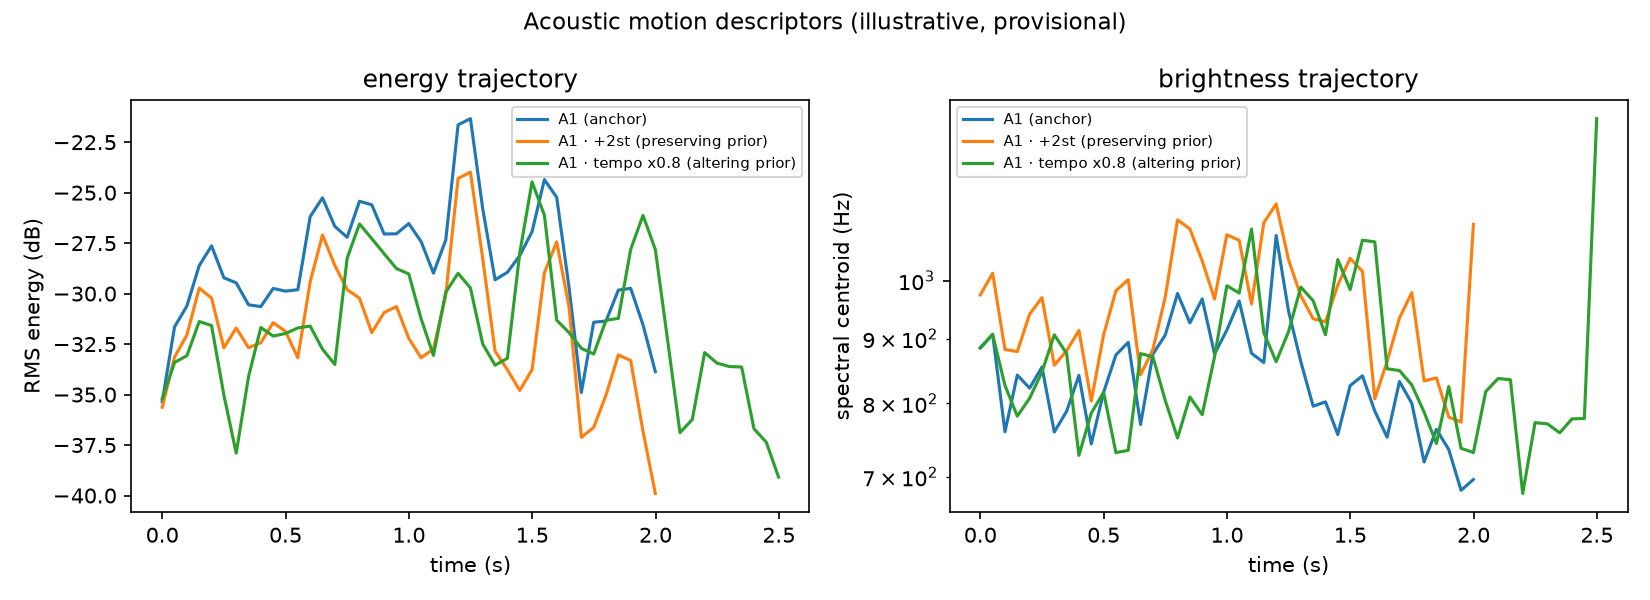
\includegraphics[width=\linewidth]{figures/pilot_motion.png}
\caption{Acoustic motion descriptors for one anchor and two of its realizations
(illustrative; provisional ontology). Left: short-time RMS energy over time;
right: spectral centroid (brightness) over time. Transposition (\texttt{+2st})
preserves the energy shape and raises the brightness curve; the strong tempo
change (\texttt{x0.8}) preserves the shape while changing the duration. This
motivates the trajectory view but is not a representation result.}
\label{fig:motion}
\end{figure}

\subsection{Human ontology validation}
\label{sec:ontology}
\paragraph{Task.} For each anchor $A$ and variant $B=T(A)$, a rater answers one
question on a 7-point scale: ``A and B are two versions of the same musical
excerpt. Rate how similar $B$'s musical motion is to $A$'s, from 1 (very
different) to 7 (same motion).'' The prompt is fixed and names exactly one
construct (T6). Anchors and variants are presented in a static HTML page with
in-page audio, so the study needs no server and works from \texttt{file://}.

\paragraph{Aggregation.} Responses are grouped by setting
$k=(\text{transform},\psi)$. For each $k$ we compute the mean, a bootstrap 95\%
CI \citep{efron1993bootstrap}, the per-response category distribution
\begin{equation}
\pi_k(c) = \frac{1}{|R_k|}\sum_{r\in R_k}\ind\!\left[\mathrm{cat}(r)=c\right],
\qquad c \in \{\text{preserving},\text{ambiguous},\text{altering}\},
\end{equation}
where $\mathrm{cat}(r)=\text{preserving}$ if $r\ge \text{mid}+\text{margin}$,
$\text{altering}$ if $r\le \text{mid}-\text{margin}$, else $\text{ambiguous}$, and
agreement via Krippendorff's ordinal $\alpha$ \citep{krippendorff2004content} and,
for complete designs, Fleiss' $\kappa$ \citep{fleiss1971measuring}.

\paragraph{Classification.} With $\text{mid}=4.0$, $\text{margin}=0.5$, minimum
raters $R_{\min}$, minimum trials $N_{\min}$, and minimum agreement
$\alpha_{\min}$:
\begin{equation}
\text{status}(k)=
\begin{cases}
\text{uncertain} & \text{if } n_{\text{raters}}<R_{\min} \text{ or } n_{\text{trials}}<N_{\min} \text{ or } \alpha_k<\alpha_{\min},\\[2pt]
\text{preserving} & \text{else if } \mathrm{CI}^{\text{lo}}_k \ge \text{mid}+\text{margin},\\[2pt]
\text{altering} & \text{else if } \mathrm{CI}^{\text{hi}}_k \le \text{mid}-\text{margin},\\[2pt]
\text{ambiguous} & \text{otherwise.}
\end{cases}
\end{equation}
A transform is \texttt{mixed} if its settings disagree. The ontology records raw
distributions, so downstream choices are auditable. Two properties matter:
\texttt{uncertain} settings are excluded from the invariance decision, and the
ontology is computed \emph{before} any representation is evaluated, breaking the
circularity of using model output to define the construct.

\subsection{Representations}
We compare four frozen encoders and one learned model: (1) \emph{handcrafted}:
per-frame RMS, spectral centroid, spectral bandwidth, zero-crossing rate, onset
strength, and $f_0$ (\texttt{pyin}), z-scored per dimension; (2) \emph{log-mel}:
64-bin frames at a fixed hop; (3) \emph{frozen MERT} \citep{li2024mert}: mid-layer
hidden states mean-pooled to a fixed rate; (4) \emph{frozen CLAP}
\citep{elizalde2023clap,wu2023laionclap}: windowed audio embeddings; and (5) a
\emph{learned trajectory}: a frozen frame encoder, then a 1D temporal transformer
\citep{vaswani2017attention} with sinusoidal positional encoding,
$d_{\text{model}}=128$, two layers, four heads, and a projection to
$z_t\in\R^{64}$. The small learned model is deliberate: H1--H3 concern the geometry
and dynamics of the representation, not encoder capacity, and a small model makes
architecture/objective ablations attributable (T5).

\subsection{Distances and geometry}
As defined in Sections~2.4--2.5. For invariance (E4) we compare,
per setting, $d(z_A,z_{T(A)})$ against cross-excerpt distances $d(z_A,z_B)$, and
summarize by the AUC of the preserving-vs-other split and the mean gap. For human
alignment (E3) we report RSA and triplet accuracy.

\subsection{Objectives}
Let $z=g_\theta(f_\phi(x))$ and $z^{+}=g_\theta(f_\phi(T(x)))$ for a setting
validated as preserving. The loss is
\begin{equation}
\mathcal{L} = \lambda_{\text{var}}\ell_{\text{var}} + \lambda_{\text{cov}}\ell_{\text{cov}} + \lambda_{\text{inv}}\ell_{\text{inv}} + \lambda_{\text{pred}}\ell_{\text{pred}} + \lambda_{\text{tri}}\ell_{\text{tri}}.
\end{equation}
With $\gamma=1$ and $C=\mathrm{Cov}(z)$,
\begin{align}
\ell_{\text{var}}(z) &= \frac{1}{d}\sum_{j=1}^{d}\max\!\left(0,\gamma-\sqrt{\mathrm{Var}(z_{\cdot j})+\epsilon}\right),\\
\ell_{\text{cov}}(z) &= \frac{1}{d}\sum_{i\ne j} C_{ij}^2, \\
\ell_{\text{inv}}(z,z^{+}) &= \lVert z-z^{+}\rVert_2^2, \\
\ell_{\text{pred}} &= \frac{1}{\sum_i w_i}\sum_{i=1}^{k} w_i\,\lVert z_{t+i}-\hat z_{t+i}\rVert_2^2, \quad w_i = 1/i, \\
\ell_{\text{tri}} &= \max\!\left(0,\lVert z_a-z_p\rVert_2-\lVert z_a-z_n\rVert_2+m\right).
\end{align}
Continuity is implemented \emph{only} through $\ell_{\text{pred}}$. We do not add a
term penalizing $\lVert z_t-z_{t+1}\rVert$, because that term is minimized by the
constant encoder of T3; predictability is the correct expression of continuity.
The variance/covariance terms follow VICReg \citep{bardes2022vicreg} and the
alignment--uniformity view \citep{wang2020alignment}; the triplet term follows
metric learning \citep{schroff2015facenet}.

\subsection{Experiments}
\begin{table}[t]
\centering
\small
\begin{tabular}{@{}llll@{}}
\toprule
ID & Experiment & Question & Criterion \\
\midrule
E1 & Transformation validation & Which settings preserve motion? & input to all \\
E2 & Collapse diagnostics & Is the representation non-degenerate? & C1 \\
E3 & Human similarity (RSA/triplet) & Does model geometry match humans? & C4 \\
E4 & Invariance & Are preserving settings close? & C2 \\
E5 & Specificity & Are altering settings separated? & C3 \\
E6 & Multi-step prediction & Structure beyond smoothness? & C5 \\
E7 & Architecture ablation & transformer vs.\ GRU vs.\ mean-pool & attribution \\
E8 & Objective ablation & contribution of var/cov/inv/pred/tri & attribution \\
\bottomrule
\end{tabular}
\caption{Experiment matrix.}
\label{tab:experiments}
\end{table}

\subsection{Local editing (deferred)}
H4 requires an inverse map from trajectory to audio---the generative component we
have not built---so editability cannot yet be tested. A decoder-free proxy is
possible (retrieval: does the nearest actual segment realize an edited
$z$-segment?), but it is not equivalent to editing and is not counted as evidence
for H4.

\begin{figure}[t]
\centering
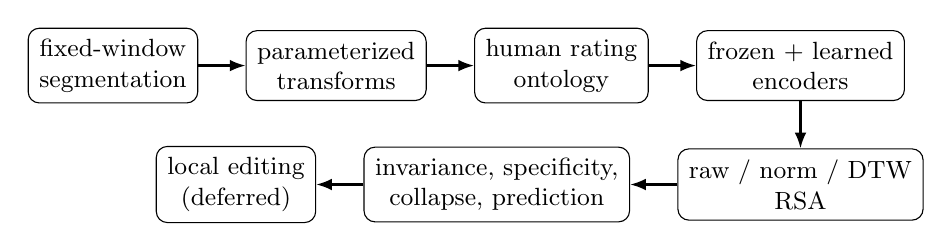
\begin{tikzpicture}[
  node distance=6mm,
  box/.style={draw, rounded corners, align=center, font=\small, inner sep=4pt},
  arr/.style={-{Latex[length=2mm]}, thick}
]
\node[box] (seg) {fixed-window\\segmentation};
\node[box, right=of seg] (tr) {parameterized\\transforms};
\node[box, right=of tr] (hum) {human rating\\ontology};
\node[box, right=of hum] (enc) {frozen + learned\\encoders};
\node[box, below=of enc] (dist) {raw / norm / DTW\\RSA};
\node[box, left=of dist] (crit) {invariance, specificity,\\collapse, prediction};
\node[box, left=of crit] (edit) {local editing\\(deferred)};
\draw[arr] (seg) -- (tr);
\draw[arr] (tr) -- (hum);
\draw[arr] (hum) -- (enc);
\draw[arr] (enc) -- (dist);
\draw[arr] (dist) -- (crit);
\draw[arr] (crit) -- (edit);
\end{tikzpicture}
\caption{Phase~1 pipeline. Transformation semantics are fixed by humans before any
representation is evaluated; editing is downstream of the preregistered criteria.}
\label{fig:pipeline}
\end{figure}

\section{Preregistered criteria and statistical plan}
\label{sec:criteria}
A representation is reported as evidence only if \emph{all} criteria hold on
held-out data.
\begin{itemize}
  \item \textbf{C1 (health).} $\mathrm{mean}_j\,\mathrm{Var}(z_{\cdot j})>v_{\min}$
  and $\effrank(z)>r_{\text{frac}}\,d$, with $v_{\min}=10^{-3}$,
  $r_{\text{frac}}=0.1$, and
  $\effrank(z)=\exp H(\sigma/\lVert\sigma\rVert_1)$ over singular values $\sigma$.
  \item \textbf{C2 (invariance).} For every setting with status \texttt{preserving},
  $\mathrm{mean}\,d(z_A,z_{T(A)})<\mathrm{mean}\,d(z_A,z_B)$ over different
  excerpts, and separation AUC $>0.5$ under $d_{\text{norm}}$.
  \item \textbf{C3 (specificity).} Settings with status \texttt{altering} yield
  distances clearly above preserving ones (same separation analysis).
  \item \textbf{C4 (human alignment).} Triplet accuracy exceeds MERT, CLAP, and
  handcrafted features under the same distance.
  \item \textbf{C5 (prediction).} Multi-step MSE is lower than persistence,
  linear extrapolation, ridge on frozen features, and constant mean.
\end{itemize}
\textbf{Decision rule.} If C1 fails, no other claim is made. If C2 fails for a
\texttt{preserving} setting, it is reclassified \texttt{ambiguous} and the
protocol re-run (a data-driven ontology update, not a metric change). If C4 fails,
the gesture ontology is reported as \emph{unsupported at this stage}, and the
failure documented rather than hidden.

\textbf{Statistical plan.} Agreement is reported per setting. Invariance uses
bootstrap CIs over excerpt pairs; human alignment uses bootstrap CIs over
triplets. For E7--E8 we report paired bootstrap intervals across seeds. Because
many settings are tested, we report the full family rather than a single best
setting, and we never select on the test split.

\section{Pilot}
\label{sec:pilot}
\textbf{Data.} Forty solo-piano excerpts from MAESTRO \citep{hawthorne2019maestro}
(train split), composer-stratified, totaling 334 minutes. We selected a mirror
storing extracted \texttt{.wav} files that match MAESTRO's official metadata paths;
audio is not redistributed and only the subset manifest is versioned.

\textbf{Stimuli.} Segmentation at $\{1,2,4\}$\,s, $50\%$ hop, at most four segments
per excerpt, 22.05\,kHz mono: \textbf{160 segments}; parameterized transforms yield
\textbf{1{,}600 variants} (10 settings per segment).

\textbf{Human study.} A dependency-free static HTML page presents \textbf{400
rating trials} (40 per setting) with in-page audio and JSON export; multiple raters
are merged before scoring. The minimum is five raters for an ontology to count as
validated.

\textbf{Baselines and models.} Handcrafted acoustic features, log-mel, frozen MERT,
frozen CLAP (weights not redistributed), and the learned trajectory. Compute is a
single CPU workstation.

\textbf{Artifacts.} \texttt{segments.jsonl}, \texttt{variants.jsonl},
\texttt{transformation\_validation.html}, a trials JSON, per-rater response JSONs,
and \texttt{ontology.json}.

\section{Preliminary engineering validation (not evidence)}
This section reports pipeline correctness only; all numbers use the provisional
priors of Table~\ref{tab:transforms} and are \emph{not} evidence about musical
motion. The unit-test suite passes on synthetic audio (segmentation and
transforms; metrics including Fleiss' $\kappa$, Krippendorff's $\alpha$, RSA, and
collapse diagnostics; losses; distances; the rating and triplet flows; experiment
drivers): 30 tests. On the 160 real segments and 1{,}600 variants, the pipeline
generates the 400-trial study and runs the frozen baselines without error. Under
the provisional ontology, on a 40-segment subset, log-mel frames give separation
AUC $0.973$ and handcrafted features $0.999$, with healthy collapse diagnostics
for both. These approach the ceiling that \emph{any} reasonable representation
reaches under an assumed ontology; they quantify the inflation described by T1 and
are the strongest argument for making the human ontology the blocking step. We
intentionally do not interpret them.

\begin{figure}[t]
\centering
\begin{minipage}{0.48\linewidth}\centering
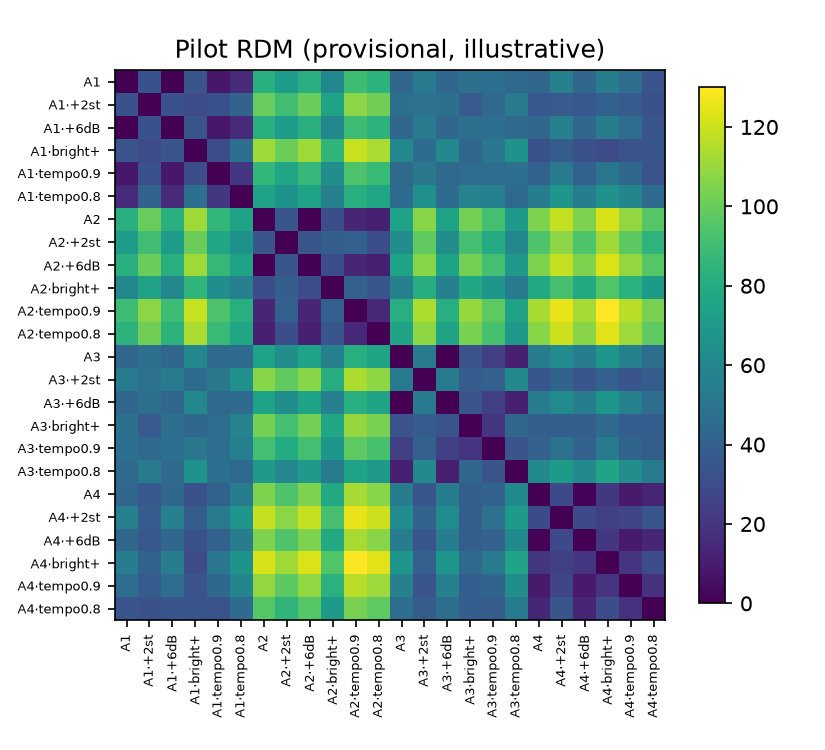
\includegraphics[width=\linewidth]{figures/pilot_rdm.png}
\end{minipage}\hfill
\begin{minipage}{0.48\linewidth}\centering
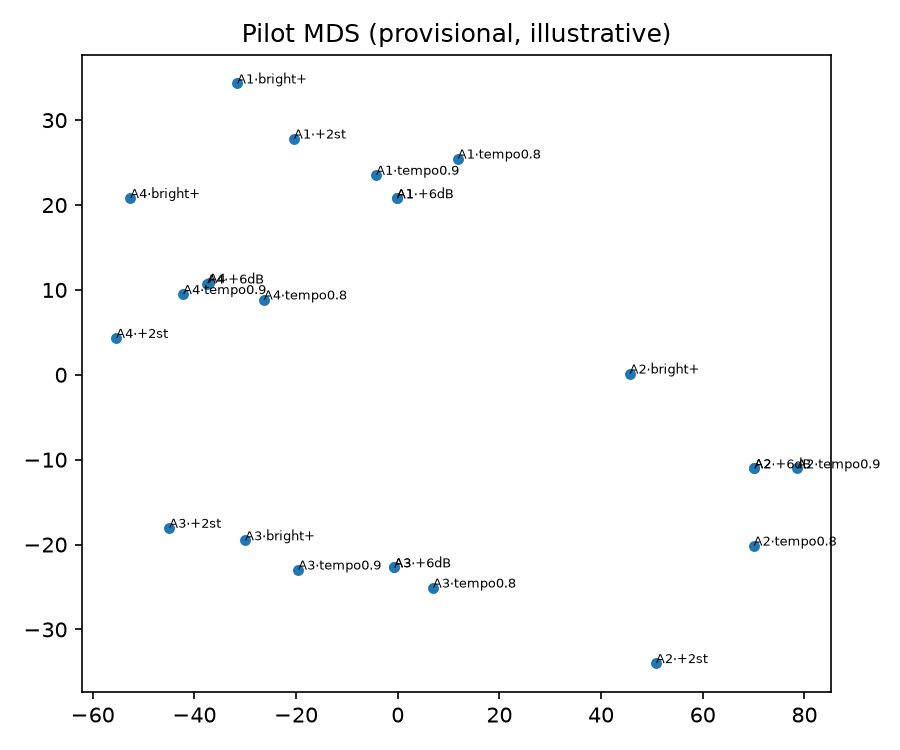
\includegraphics[width=\linewidth]{figures/pilot_mds.png}
\end{minipage}
\caption{Latent geometry of the pilot under the provisional ontology
(log-mel pooled embeddings; illustrative, not evidence). Left: pairwise distance
matrix over four anchors (\texttt{A1}--\texttt{A4}) and their variants. Right:
metric MDS of the same embeddings. Within-anchor variants form blocks and
clusters, while cross-anchor distances are larger, and the two tempo settings
span a wide range---consistent with the \texttt{mixed} prior and with the need to
estimate the tempo boundary from humans.}
\label{fig:pilot_geometry}
\end{figure}

\section{Limitations and threats to validity}
The central limitation is that the human ontology has not been collected, so
H1--H4 are untested and every invariance number is provisional. The timbre
transform is a high-shelf proxy, and articulation changes are absent because they
need note-level (MIDI) edits. The pilot is solo piano by design; generalization to
polyphony, voice, and multi-instrument music is untested and may change what
``motion'' means. Frozen MERT and CLAP are implemented but were not run in the
pilot, so the human-alignment comparison is incomplete. The distance choice and
the classification margin are conventions; the ontology schema records raw
distributions so they can be probed post hoc. Fixed-window segmentation may bias
the candidate gestures; it is chosen to protect the ontology, not because it is
optimal.

\section{Open-source release and reproducibility}
\label{sec:release}
The repository contains segmentation and transforms, the human-study runner,
parameterized ontology scoring, metrics, representation and baseline encoders,
losses, experiment drivers, visualization, and the preregistered criteria and
protocol, and is available at \url{https://github.com/Fengrru/mmt}.
Reproduction is a short sequence of commands
(\texttt{docs/reproduction.md}). Code is MIT-licensed; MAESTRO audio is subject to
its own license (CC BY-NC-SA 4.0) and is not redistributed. The release includes a
\texttt{CONTRIBUTING.md} whose first rule is that model results must never define
the ontology, preserving the identification argument for downstream contributors.

\section{Conclusion}
We argued that the difficulty in learning a musical-motion trajectory is
identification, not capacity, and converted that concern into a preregistered
protocol and an open implementation. The framework derives its design from six
concrete threats and is constructed so that a degenerate shortcut fails at least
one mandatory criterion. Its value does not depend on the hypothesis being true:
if human ratings show the assumed transformations do not preserve motion, or if a
simple acoustic baseline already matches the human construct, the framework
reports this cleanly and early, before any generative system is built. We release
the pilot and protocol so the human study can be run and, if warranted, the
hypothesis falsified.

\appendix
\section{Ontology schema}
\begin{verbatim}
{
  "validated": true,
  "scale": 7, "midpoint": 4.0, "margin": 0.5,
  "entries": [{
    "key": "time_stretch:rate=0.9",
    "transform": "time_stretch",
    "params": {"rate": 0.9},
    "n_ratings": 48, "n_raters": 6, "n_trials": 8,
    "mean": 6.0, "ci_low": 5.7, "ci_high": 6.3,
    "judgment": {"preserving": 1.0, "ambiguous": 0.0, "altering": 0.0},
    "agreement": {"krippendorff_alpha_ordinal": 0.67, "fleiss_kappa": 0.6},
    "status": "preserving"
  }],
  "by_key": {"time_stretch:rate=0.9": "preserving"},
  "by_transform": {"time_stretch": "mixed"}
}
\end{verbatim}

\section{Latent shared projection (provisional)}
\begin{figure}[h]
\centering
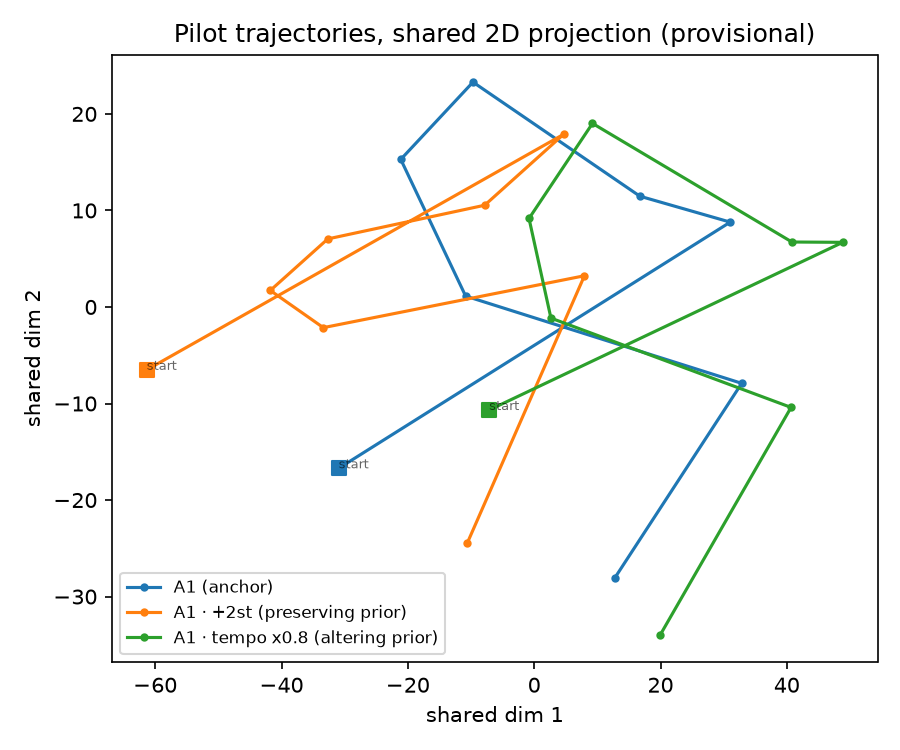
\includegraphics[width=0.72\linewidth]{figures/pilot_trajectories.png}
\caption{Shared 2D PCA projection of one anchor and two realizations
(log-mel frames, coarse to eight time steps; illustrative). A single projection
basis is fit on all frames so trajectories are comparable. The high-dimensional
frame trajectory is deliberately not used as a primary figure; the geometry of
representation is summarized by the RDM/MDS (Figure~\ref{fig:pilot_geometry}),
while interpretable motion is shown in Figure~\ref{fig:motion}.}
\label{fig:pilot_latent}
\end{figure}

\section{Reporting checklist}
For every reported number state: (i) the distance used; (ii) the ontology status of
every setting involved; (iii) agreement and $n$; (iv) whether \texttt{validated} is
true; (v) collapse diagnostics; (vi) all baselines. A number that omits any of
these is not part of the claim.

\bibliographystyle{plainnat}
\bibliography{references}

\end{document}
